\documentclass[12pt]{report}
\usepackage[a4paper, margin=3cm]{geometry}
\usepackage{anyfontsize}
\usepackage{setspace}
\usepackage[dvipsnames]{xcolor}
\usepackage[utf8]{inputenc}
\usepackage{ragged2e}
\usepackage{svg}
\usepackage{tikz}
\usepackage{titlesec}
\usepackage[hidelinks]{hyperref}
\usepackage{tabularray}
\usepackage{array}
\usepackage{amsmath}
\usepackage{amsfonts}
\usepackage{multicol}
\usepackage{fancyvrb}
\usepackage{amsmath}
\usepackage{algorithm}
\usepackage[noend]{algpseudocode}
\usepackage[edges]{forest}
% \usepackage[
%     backend=biber,
%     style=numeric,
%     sorting=none
% ]{biblatex}
% \addbibresource{references.bib}
\graphicspath{ {images/} }

\usepackage[T1]{fontenc} % to correctly display <, > and | symbols

\makeatletter         
\renewcommand\maketitle{{
    {\hfill \LARGE  \@author} \\[4ex]
    
    \begin{raggedright}
    
        {\setlength{\parindent}{0pt} \fontsize{40}{20} \renewcommand{\baselinestretch}{2} \bfseries \@title \par}

        \vspace{4ex}

        \begin{spacing} {0.25}
            \noindent\rule{\linewidth}{0.4pt} 
            \noindent\rule{\linewidth}{0.4pt}
        \end{spacing}

        \vspace{4ex}
        
        \LARGE Computer Science Tripos Part II

        \LARGE Gonville and Caius College
        
        \LARGE \@date
        
    \end{raggedright}
        
}}
\makeatother

\title{Implementing the HotStuff consensus algorithm}
\author{Marc Harvey-Hill}
\date{March 2023}

\titleformat{\chapter}[display]
  {\bfseries\Huge}
  {\filleft\Large\chaptertitlename~\thechapter}
  {0ex}
  {}
  [\vspace{-\baselineskip}\noindent\rule{\linewidth}{0.4pt}\vspace{-\baselineskip}]

\begin{document}

\begin{titlepage}
    \maketitle

    \vfill

    \noindent
\includegraphics[scale=0.1]{university.png}

    \tikz[remember picture,overlay] \node[opacity=0.3,inner sep=0pt] at (current page.center){
\includegraphics[width=\paperwidth,height=\paperheight]{featured_image.jpeg}};
\end{titlepage}

\setlength{\parskip}{\baselineskip}

\chapter*{Declaration of Originality}

I, Marc Harvey-Hill of Gonville and Caius College, being a candidate for Part II of the Computer Science Tripos, hereby declare that this dissertation and the work described in it are my own work, unaided except as may be specified below, and that the dissertation does not contain material that has already been used to any substantial extent for a comparable purpose. I am content for my dissertation to be made available to the students and staff of the University.

\noindent Signed [signature]

\noindent Date [date]

\tableofcontents

\setcounter{chapter}{1}
\chapter*{Introduction}
\addcontentsline{toc}{chapter}{Introduction}

% The introduction should explain the principal motivation for the project and show how the work fits into the broad area of surrounding computer science and give a brief survey of previous related work. It should generally be unnecessary to quote at length from technical papers or textbooks. If a simple bibliographic reference is insufficient, consign any lengthy quotation to an appendix.

Blockchains promise to decentralise applications that were traditionally run in a centralised manner. The implications of this are far-reaching: central banks can be replaced by decentralised cryptocurrencies \cite{nakamotoBitcoinPeertoPeerElectronic2008,perniceCryptocurrency2021}, traditional corporations can be replaced with decentralised autonomous organisations (DAOs) \cite{hassanDecentralizedAutonomousOrganization2021,ethereumWhite}, internet infrastructure like DNS servers can be decentralised \cite{EthereumNameService}, and any possible algorithm can be run on a decentralised `world computer' \cite{ethereumWhite,ethereumYellow}. The innovation that makes blockchains possible is the byzantine consensus algorithm.

Byzantine fault-tolerant consensus algorithms allow a group of parties to agree on some piece of information under adverse conditions where some messages can be lost and some parties are controlled by a malicious adversary. For example, one could create a cryptocurrency by using such an algorithm to reach consensus on a ledger of transactions like ``Account Alice transfers account Bob £10''; the algorithm will ensure that transactions cannot be lost and the system cannot be sabotaged by malicious actors.

Byzantine consensus algorithms can be viewed as solutions to the byzantine generals problem \cite{lamportByzantineGeneralsProblem1982}, in which malicious actors are represented by byzantine generals. Here, a group of generals must all agree to siege a castle at the same time, but they can only communicate via messengers that take some time to arrive and can be captured en route. Additionally, up to a third of the generals may be malicious, and try to prevent the other generals from reaching consensus on a time to attack. By following a byzantine consensus protocol the generals can reach consensus on a value like ``attack at dawn''. Multi-valued consensus algorithms allow consensus to be reached on multiple values, resulting in a continuously growing log that can never be modified or erased, only extended. This problem statement assumes that the number of participating generals is fixed.

Blockchains can be either permissioned, or permissionless. Permissioned blockchains have a previously agreed set of participants in the consensus algorithm, whereas permissionless blockchains allow participants to join and leave freely. Most well-known blockchains, such as Bitcoin \cite{nakamotoBitcoinPeertoPeerElectronic2008} and Ethereum \cite{ethereumWhite, ethereumYellow}, are of the permissionless variety. Permissioned blockchains can be deployed in a permissionless setting if they are augmented with an additional layer of security, which can be proof of work, proof of stake, or some other similar mechanism. These aim to prevent a `Sybil attack' where a large number of malicious nodes join the network, exceeding the threshold that only one-third of nodes can be malicious. For example, proof of work adds a requirement for proof of computational work to participate in consensus, making Sybil attacks economically and computationally infeasible. Permissioned blockchains are of interest for applications within a group or organisation, such as a company, where the participating nodes are known in advance.

HotStuff is a byzantine consensus algorithm that was notably used by Meta's Libra \mbox{project \cite{baudetStateMachineReplication2019}}, a cancelled permissioned blockchain-based payments system. The algorithm is relevant because of various performance advantages over other byzantine consensus algorithms such as PBFT \cite{castroPracticalByzantineFault1999}, SBFT \cite{golanguetaSBFTScalableDecentralized2019}, DLS \cite{dworkConsensusPresencePartial1988}, Tendermint \cite{kwonTendermintConsensusMining2014}, and Casper \cite{buterinCasperFriendlyFinality2019}.

Building practical, well-performing implementations of consensus algorithms is non-trivial. These algorithms are usually given in short pieces of pseudocode that may not be specified precisely and require much more code to implement in practice. Such software has a wide range of failure modes mostly due to their parallel nature, including deadlocks, resource starvation, and bugs in the implementation \cite{chandraPaxosMadeLive2007}.

The main contributions of this dissertation are:
\begin{itemize}
	\item Giving a complete specification and proof of HotStuff (Section~\ref{spec}), that adapts the pacemaker mechanism, which was not specified in the original paper. This specification synthesises the chained algorithm described in the paper (Section~\ref{chaining}), a view-change protocol based on other talks and papers (Section~\ref{viewchange}), and my changes to integrate the pacemaker with HotStuff without the need for synchronised clocks.
	\item Providing a reference implementation of HotStuff in OCaml based on a paper by Yin et. ~al~ \cite{yinHotStuffBFTConsensus2019}.
	\item Giving solutions to key practical challenges of implementation and optimisations that can be made (Section~\ref{performance}), as well as showing their effectiveness (Section~\ref{ablation}).
	\item Synthesising information from different sources to provide a complete explanation of the HotStuff algorithm, and how it can be arrived at through modifications to simpler consensus algorithms (basic algorithm Section~\ref{hotstufftheory}, chained algorithm Section~\ref{chaining}, pacemaker Section~\ref{pacemaker}).
\end{itemize}

\stepcounter{chapter}
\chapter*{Preparation}
\addcontentsline{toc}{chapter}{Preparation}

% Principally, this chapter should describe the work which was undertaken before code was written, hardware built or theories worked on. It should show how the project proposal was further refined and clarified, so that the implementation stage could go smoothly rather than by trial and error.

% Throughout this chapter and indeed the whole dissertation, it is essential to demonstrate that a proper professional approach was employed.

% The nature of this chapter will vary greatly from one dissertation to another but, underlining the professional approach, this chapter will very likely include a section headed "Requirements Analysis" and refer to appropriate software engineering techniques used in the dissertation. The chapter will also cite any new programming languages and systems which had to be learnt and will mention complicated theories or algorithms which required understanding.

% It is essential to declare the starting point. This states any existing codebase or materials that your project builds on. The text here can commonly be identical to the text in your proposal, but it may enlarge on it or report variations. For instance, the true starting point may have turned out to be different from that declared in the proposal and such discrepancies must be explained.

In this chapter, I disclose my experience before beginning this project (Section~\ref{start}), explain the HotStuff algorithm by building up from simpler consensus algorithms (Section~\ref{hotstufftheory}), outline the tools and libraries (Section~\ref{tools}) that were used, highlight requirements that the implementation should meet (Section~\ref{requirements}), and describe the professional methodology (Section~\ref{softwareeng}) that was employed during implementation.

\section{Starting point} \label{start}
Although I had some experience using OCaml through the IA Foundations of Computer Science course, I had never utilized it in a project before. The IB Distributed Systems course provided some useful background knowledge, particularly as it briefly covered Raft~\cite{ongaroSearchUnderstandableConsensus2014}, a non-byzantine consensus algorithm. Additionally, I had a basic understanding of byzantine consensus from my reading into Nakamoto consensus~\cite{nakamotoBitcoinPeertoPeerElectronic2008} and from developing a wallet application for Ethereum~\cite{ethereumWhite, ethereumYellow}; neither of these was directly useful to implementing HotStuff, but they gave me some wider context of the field.

\section{HotStuff algorithm} \label{hotstufftheory}
HotStuff~\cite{yinHotStuffBFTConsensus2019} is a byzantine consensus algorithm; it allows a group of nodes to reach consensus on a log of values under adverse conditions, such as messages being lost, or some nodes acting maliciously (byzantine). In each view, a leader node proposes some value by sending it to the replicas (another word for nodes). After several messages are exchanged a prefix of the log may be committed, meaning there is consensus on that part of the log and it is immutable.

The system model describes the adverse conditions under which HotStuff can operate:
\begin{assumption}[Partially Synchronous] \label{partialsyncassumption}
	Messages sent by one party will always be delivered to another within some bounded amount of time ($\Delta$) after global synchronisation time (GST) has been reached~\cite{dworkConsensusPresencePartial1988}.
\end{assumption}

\begin{assumption}[Authenticated] \label{authassumption}
	We assume that all messages are signed, providing an authenticated channel where no messages can be spoofed.
\end{assumption}

\begin{assumption}[Byzantine] \label{byzassumption}
	A maximum of $f$ faulty nodes may be controlled by an adversary, where $n = 3f + 1$ and $n$ is the total number of nodes.
\end{assumption}

Assumptions \ref{partialsyncassumption} and \ref{byzassumption} are the weakest possible assumptions under which it is possible to reach consensus~\cite{peaseReachingAgreementPresence1980,fischerEasyImpossibilityProofs1986}. Assumption \ref{authassumption} is also needed, but byzantine consensus is possible without cryptographic signatures; there is an algorithm called Information Theoretic HotStuff, that does not use signatures and is secure against a computationally unbounded adversary\footnote{An authenticated channel can be obtained without signatures by using one time pads or quantum cryptography~\cite{bennettExperimentalQuantumCryptography1992}.}~\cite{abrahamInformationTheoreticHotStuff2020}.

HotStuff has the following properties:

\begin{property}[Safety] \label{safetyproperty}
	Once some prefix of a log has been committed, that part of the log is immutable, it can only be appended to.
\end{property}

\begin{property}[Liveness] \label{livenessproperty}
	Assuming there is a functioning pacemaker, the system is guaranteed to make progress within some bounded amount of time once GST has been reached and a non-faulty leader is chosen. The pacemaker ensures that the honest replicas will be in views with an honest leader for long enough to make progress (Section~\ref{pacemaker}).
\end{property}

\begin{property}[Optimistic Responsiveness] \label{optresponsiveproperty}
	Once GST has been reached and a non-faulty leader is chosen, the system can make progress as fast as network conditions allow; it does not have to wait for some timeout to elapse~\cite{passThunderellaBlockchainsOptimistic2018}.
\end{property}

Basic HotStuff is a responsive byzantine consensus algorithm (Section~\ref{optresponsive}). A simpler consensus algorithm that is neither responsive nor byzantine is described in Section~\ref{nonbyzconsensus}. This algorithm is then extended in Section~\ref{byzconsensus} to handle byzantine threats. Finally, Section~\ref{optresponsive} explains how the algorithm is made responsive by removing the need for a timeout to progress, arriving at the basic HotStuff algorithm.

\subsection{Non-byzantine consensus} \label{nonbyzconsensus}
In this section, a generic algorithm is described to solve the problem of reaching consensus with a crash-stop model, which assumes that nodes cannot be malicious but can crash and never come back online. Examples of similar algorithms include Raft~\cite{ongaroSearchUnderstandableConsensus2014} and \mbox{MultiPaxos~\cite{lamportParttimeParliament1998, lamportPaxosMadeSimple2001}}.

Each view is composed of several phases. In each phase, the leader broadcasts to the replicas, that respond with an acknowledgement (ack). The leader waits until it receives a quorum of acks before proceeding to the next phase; for this algorithm, a quorum consists of $\lceil\frac{n}{2}\rceil$ acks.

Consensus can be used in state machine replication~\cite{lamportTimeClocksOrdering1978,schneiderImplementingFaulttolerantServices1990}. In this setting, the nodes reach consensus on a log of commands that have been sent by a client. Once a prefix of the log is committed the client can be responded to and the committed commands are executed in order, ensuring that all nodes will be in the same state.

In this generic algorithm, each view consists of three phases:

\begin{description}
	\item \textit{new-view} --- all replicas send a \textit{new-view} message to the leader, containing their longest previously committed log.
	\item \textit{commit} --- once the leader receives a quorum of $\lceil\frac{n}{2}\rceil$ \textit{new-view} messages, it picks the longest log ($\lambda$) to propose. It then broadcasts a \textit{commit} message to the replicas, proposing $\lambda'$ to the nodes, where $\lambda'$ is $\lambda$ optionally extended with the leader's new value. The replicas send a \textit{commit} ack.
	\item \textit{decide} --- once the leader receives a quorum of acks, the log has been successfully committed. The leader can broadcast ``decide'' to the replicas, who can execute the new commands and respond to the client. The replicas send a \textit{new-view}, beginning the next view.
\end{description}

Crucially, this algorithm is safe (Property \ref{safetyproperty}). Since the leader waits to receive a quorum of greater than $\lceil\frac{n}{2}\rceil$ \textit{new-view} messages, $\lambda$ is guaranteed to be the longest log that has previously been committed. This is because the quorum of \textit{new-view} messages must share at least one node with the past quorum of \textit{commit} acks for $\lambda$. The new proposal $\lambda'$ will never conflict with $\lambda$, hence the algorithm is safe.

\subsection{Byzantine consensus} \label{byzconsensus}
In this section, consensus under a byzantine system model (Assumption \ref{byzassumption}) is achieved by extending the non-byzantine algorithm introduced in Section~\ref{nonbyzconsensus}. This is accomplished by first introducing the quorum certificate (QC), a cryptographic proof that a leader has received a quorum of acks. Next, the threats posed by byzantine nodes are considered, and a generic algorithm that solves these problems is presented, along with an argument for safety. Examples of similar algorithms include Tendermint~\cite{kwonTendermintConsensusMining2014} and Casper~\cite{buterinCasperFriendlyFinality2019}.

\subsubsection{Quorum certificates}

A QC is a quorum of $n - f$ acks with a matching threshold signature. A threshold signature combines several signatures of the same message into one~\cite{shoupPracticalThresholdSignatures2000, cachinRandomOraclesConstantinople2005}; in this case, the signature from each ack is combined\footnote{Recall that messages are signed to provide authenticated delivery (Assumption \ref{authassumption}).}. QCs have a key property that the byzantine algorithm will rely on:

\begin{property} \label{qcproperty}
There will always be at least one honest node in the intersection of any two QCs.
\end{property}

Recall that $n = 3f + 1$. The property holds since a QC contains a quorum of $n - f = 2f + 1$ acks, of which at least $f + 1$ must be from honest nodes. To have two quorums that do not share an honest node would require at least $2(f + 1) = 2f + 2$ honest nodes, but the system only has $2f + 1$.

\subsubsection{Threats introduced by byzantine nodes}
Two threats are introduced by Byzantine nodes, which will be dealt with in turn. Solutions to these threats are presented; their effectiveness will become clear in the argument for the safety of the algorithm.

\begin{threat}[Equivocation] \label{threat1}
A faulty leader proposes one value to some replicas and a different value to others. For example, in the case of a cryptocurrency a malicious actor (Mallory) could carry out a double-spend attack by proposing ``Mallory transfers Alice £10'' to some nodes and ``Mallory transfers Bob £10'' to others, even if Mallory's account contains less than £20.
\end{threat}

Solution --- add a new stage \textit{prepare} which happens just before the \textit{commit} phase, where the leader pre-proposes a log before proposing it in the \textit{commit} phase.\\

\begin{threat} \label{threat2}
A faulty leader proposes a log that conflicts with one that has previously been committed.
\end{threat}

Solution --- make replicas \textit{lock} on a proposal once they receive a \textit{commit} message, and not accept a pre-proposal for a conflicting log.

\subsubsection{Byzantine fault-tolerant algorithm}
Modifying the non-byzantine algorithm (Section~\ref{nonbyzconsensus}) to include solutions to Threat \ref{threat1} and \ref{threat2} results in the following:

\begin{description}
	\item \textit{new-view} --- \textit{unchanged.}
	\item \textit{prepare} --- the leader waits $\Delta$ until it receives a \textit{new-view} message from all replicas (this will be revisited in Section~\ref{optresponsive}), and then picks the longest log it received ($\lambda$) to pre-propose. It then broadcasts a \textit{prepare} message to the replicas, pre-proposing $\lambda'$ to the nodes, where $\lambda'$ is $\lambda$ optionally extended with the leader's new value. The replicas ensure that $\lambda'$ does not conflict with their \textit{lock} before sending an ack.
	\item \textit{commit} --- the leader waits until it receives a quorum of \textit{prepare} acks. It then broadcasts a \textit{commit} message to the replicas, proposing $\lambda'$ to the nodes, and includes a QC of \textit{prepare} acks. The replicas then \textit{lock} on $\lambda'$ and send a \textit{commit} ack.
	\item \textit{decide} --- \textit{unchanged.}
\end{description}

\subsubsection{Argument for safety} \label{safetyargument}
An informal inductive argument is presented to show that the algorithm is safe (Property~\ref{safetyproperty}) based on it solving Threat \ref{threat1} and \ref{threat2}. Safety requires that if some log $\lambda$ is committed in view $v$, at no point in future will a conflicting log be committed.

Base case --- in view $v$, no log that conflicts with $\lambda$ may be committed; in other words, equivocation (Threat \ref{threat1}) is not possible. For two logs to have been committed in the same view, there must have been two QCs of \textit{prepare} acks. By Property \ref{qcproperty}, there must be at least one honest replica in the intersection of these QCs that would not have acknowledged conflicting proposals in the same view.

Inductive step --- no conflicting log can be proposed in view $v'$ where $v' > v$ (Threat \ref{threat2}). This holds because any log pre-proposed in view $v'$ must receive a QC of \textit{prepare} acks; by Property \ref{qcproperty}, there must be at least one honest node in the intersection between this QC, and the QC of \textit{commit} acks $\lambda$ in view $v$. This honest replica is locked on $\lambda$, so would not accept a proposal that conflicts with it.

From this, it follows that in no view from $v$ onwards will a log conflicting with $\lambda$ be committed, so the algorithm is safe.

\subsection{Optimistic responsiveness} \label{optresponsive}
This section presents the basic HotStuff algorithm by extending the generic byzantine consensus algorithm (Section~\ref{byzconsensus}) to make it optimistically responsive (Property \ref{optresponsiveproperty}). Optimistic responsiveness means that the system can make progress as fast as network conditions allow without waiting for a timeout, once GST has been reached~\cite{passThunderellaBlockchainsOptimistic2018}.

The byzantine consensus algorithm is not responsive as a timeout is needed in the \textit{prepare} phase. The problem that necessitates this timeout is first described, followed by the presentation of an algorithm that solves it. An informal argument is made that liveness is not broken by this algorithm.

\subsubsection{Why the timeout was necessary}
For the system to have liveness (Property \ref{livenessproperty}), the leader must wait for $\Delta$ to elapse so that it receives a \textit{new-view} message from all honest replicas before it pre-proposes a log. Consider what would happen if the leader did not wait for this timeout, and did not receive a \textit{new-view} from some honest replica $x$. $x$ may be locked on a longer log than the other replicas, as in some past view it received the \textit{commit} message, but other replicas did not\footnote{N.B. this means that the value was never actually committed, as this would have required a quorum of \textit{commit} acks}. When the leader sends the \textit{prepare} message, $x$ will not vote the pre-proposal as it is locked on a longer log, so the leader will not acquire a quorum of acks to make progress; this breaks liveness.

Solution idea --- add a \textit{pre-commit} phase directly before the \textit{commit} phase, where replicas store a \textit{key} for a proposal that they include in their \textit{new-view} message; this removes the need for a timeout, making the algorithm responsive.

\subsubsection{Basic HotStuff algorithm}

Modifying the byzantine algorithm (Section~\ref{byzconsensus}) to include the solution idea leads to the following:

\begin{description}
	\item \textit{new-view} --- all replicas send their \textit{key} to the leader.
	\item \textit{prepare} ---  \textit{as before, but picks the key for the longest log.}
	\item \textit{pre-commit} --- the leader waits until it receives a quorum of \textit{prepare} acks. It then broadcasts a \textit{pre-commit} message to the replicas, which contains a QC of \textit{prepare} acks. The replicas store this QC as a \textit{key} and send a \textit{pre-commit} ack.
	\item \textit{commit} --- \textit{as before, but creates QC from pre-commit acks instead of prepare acks.}
	\item \textit{decide} --- \textit{unchanged.}
\end{description}

\subsubsection{Argument for liveness} \label{livenessargument}
I informally argue for the liveness (Property \ref{livenessproperty}) of the basic HotStuff algorithm.

The non-faulty leader is guaranteed to receive a \textit{key} for the longest log ($\lambda^*$) that some honest replica is locked on. This is because for some replica to become locked on $\lambda^*$ there must be at least $f + 1$ honest nodes that have a \textit{key} for $\lambda^*$. The leader must hear about $\lambda^*$ from one of these honest nodes when it receives a quorum of \textit{new-view} messages and then propose it to the replicas.

The honest replicas will vote for the proposed log $\lambda^*$ as it does not conflict with their \textit{lock} and they are in the same view. The honest replicas are guaranteed to be synchronised in the same view by the assumption that there is a functioning pacemaker (Section~\ref{pacemaker}). Furthermore, the replicas will progress through the other phases by the assumption that GST has been reached and messages must be delivered within $\Delta$.

\section{Tools \& libraries} \label{tools}
This section describes the language and libraries that were used and justifies why they were appropriate for this project. All libraries used are open source under the MIT licence.

\subsection{OCaml}
I chose OCaml~\cite{ocaml} for its high-level nature, static type system, ability to blend functional and imperative paradigms, powerful module system, and good library support, which are all suitable for implementing HotStuff. OCaml's multi-paradigm nature enables the core state machine to be expressed functionally and the RPC library to be interacted with imperatively. Its powerful module system facilitates writing highly reusable code, enabling key components like the consensus algorithm to be easily reused in other projects. Choosing a language with suitable features to aid implementation is more important than picking a "high-performance" language like C++, given that cryptography, message serialisation, and network delays are typically the performance bottlenecks for distributed byzantine algorithms.

\subsection{Lwt}
Lwt~\cite{lwt} is a concurrent programming library for OCaml. It allows the creation of promises, which are values that will become determined in the future; these promises may spawn threads that perform computation and I/O in parallel. To use Lwt I had to learn about monads, which are ways of sequencing effects in functional languages that are used by promises in Lwt.

Lwt is useful to this project as promises provide a way to asynchronously dispatch messages over the network and wait for their responses in different threads. Promises are cheap to create in Lwt, so one can create many lightweight threads with good performance.

Alternative concurrency libraries may have had better performance, namely Async~\cite{async} and EIO~\cite{eio}. I chose Lwt over these libraries due to superior documentation and stability.

\subsection{Cap'n Proto}
Cap'n Proto~\cite{capnp} is an RPC framework that includes a library for sending and receiving RPCs, serialising messages, and a schema language for designing the format of RPCs that can be sent. Benchmarks for the library are presented in Section~\ref{capnpbenchmark}.

\subsection{Tezos cryptography} \label{tezos}
The Tezos cryptography library~\cite{tezosCrypto} provides functions to sign some data using a private key, aggregate several signatures into a single one, and check whether an aggregate signature is valid. Benchmarks for the library are presented in Section~\ref{tezosbenchmark}.

The only difference from the threshold signatures needed by HotStuff is that each individual signature in an aggregate signature can sign different data, whereas with threshold signatures each individual signature is over the same data. It is trivial to implement threshold signatures using this library by checking that the data is the same for all signatures inside the aggregate signature.

\section{Requirements analysis} \label{requirements}

To be successful the implementation should conform to the following requirements:
\begin{itemize}
	\item Correctness --- the consensus algorithm should be implemented as it is described in the paper~\cite{yinHotStuffBFTConsensus2019}. This can be established by testing the program trace for compliance with the algorithm specification.
	\item Evaluation --- analysis of system throughput and latency should be carried out by testing the program locally, analysing the trace, and testing in a simulated network\footnote{The proposal (Appendix~\ref{proposal}) stated that the system should be evaluated on a simulated network of 32 nodes, but reaching this level of performance was not possible due to limitations of Cap'n Proto (Section~\ref{capnpbenchmark}).}.
	\item Optimisation --- implement features to improve transaction throughput and reduce latency over the naive implementation.%This can be achieved through architectural decisions, tuning the scheduler, and ensuring cryptographic libraries are being used efficiently.
\end{itemize}

\section{Software engineering practices} \label{softwareeng}

This section describes the professional software engineering methodology deployed during implementation and justifies why this project is ethical.

\subsection{Development methodology} \label{devmethods}

For this project, I used an iterative waterfall development methodology. Objectives were chosen per the timetable set out in the proposal (Appendix \ref{proposal}). Development then proceeded in cycles of implementation and testing to ensure compliance with the protocol specification. This approach was particularly useful during the optimisation of the system (Section~\ref{performance}), which involved extensive log analysis and rapid prototyping to compare performance.

\subsection{Testing \& debugging methodology} \label{testing}

Unit testing was carried out using `expect tests', which compare a program trace to the correct output. A testing suite of expect tests verifies that the program behaves as specified in the HotStuff paper. This suite has 100\% code coverage\footnote{The coverage report in \textit{\_coverage/index.html}, reports 98.13\% coverage, but the only code not covered is the expect tests themselves.} of the consensus state machine code.%, the coverage report is at \textit{\_coverage/index.html}.

Memtrace~\cite{memtrace} was used to profile the memory usage of the program. %One can generate a flame graph of memory allocations to see which parts of the program are using the most memory.

Mininet~\cite{mininet,lantzNetworkLaptopRapid2010} was used to test the system in a simulated wide area network (Section~\ref{minineteval}).

The distributed nature of this project meant that debugging deadlocks and performance issues had to be carried out by manual inspection of the program trace and timing sections of the program. This is because the cause of these issues is often some process waiting or a backlog of work forming on some node, but this cannot be detected by normal debugging tools and profilers that track metrics like CPU usage.

\subsection{Source code management}
I used Git for version control and regularly pushed my local changes to a GitHub repository.

\subsection{Ethical statement}
This project contributes to an existing blockchain ecosystem. Blockchains have many positive applications, but by their nature, they can facilitate the creation of exploitative markets. Since this software is already widely available, this project will not further this exploitation. Additionally, permissioned blockchains alleviate some of these harms as they are deployed in more controlled environments, and do not require energy-intensive proof of work mechanisms.

\stepcounter{chapter}
\chapter*{Implementation}
\addcontentsline{toc}{chapter}{Implementation}

% This chapter should describe what was actually produced: the programs which were written, the hardware which was built or the theory which was developed. Any design strategies that looked ahead to the testing stage should be described in order to demonstrate a professional approach was taken.

% Descriptions of programs may include fragments of high-level code but large chunks of code are usually best left to appendices or omitted altogether. Analogous advice applies to circuit diagrams or detailed steps in a machine-checked proof.

% The implementation chapter should include a section labelled "Repository Overview". The repository overview should be around one page in length and should describe the high-level structure of the source code found in your source code repository. It should describe whether the code was written from scratch or if it built on an existing project or tutorial. Making effective use of powerful tools and pre-existing code is often laudable, and will count to your credit if properly reported. Nevertheless, as in the rest of the dissertation, it is essential to draw attention to the parts of the work which are not your own. 

% It should not be necessary to give a day-by-day account of the progress of the work but major milestones may sometimes be highlighted with advantage.

% practical contributions.
% present deadlocks \& performance tests.
% reusable modules.

% Live testing revealed many subtle bugs, deadlocks, and performance issues (memory usage, messages dropped due to bugs preventing leaders from always advancing) that were time consuming to debug. However they helped me to flesh out a pacemaker algorithm based on these ad-hoc fixes that we have proven both correctness and liveness for. I also improved the ease of implementability based on practicalities I discovered during implementation (eg. using node offset and hashes to compare nodes)

\section{Overview}
Present main program structure by modules: the consensus state machine and its interface, the server code \& main loop (including stream), communication schema
% some of this is inspired by the OCons project, it was still in development
\section{Pacemaker Specification}
We present the pseudocode given in the HotStuff paper (see algorithm 4 \& 5) with our additions coloured in green and modifications in pink. We have only shown the main changes and not the other features and performance improvements we have made (such as batching), we will present these in \ref{deadlock}. In order to better map to the original pseudocode we break the algorithm into HotStuff and the pacemaker, although in our modified algorithm these two sections are not cleanly separable.

\begin{algorithm}[h!]
	\caption{Modified HotStuff}\label{hotstuff}
	\begin{algorithmic}[1]
	\color{Magenta}
	\Function{CREATE{\large L}EAF}{\textit{parent, cmd, qc}}
		\State $\textit{b.parent} \gets \text{branch extending with dummy nodes from}\ \textit{parent}\ \text{to height}\ \textit{curView}$
		\State $\textit{b.height} \gets \textit{curView} + 1$
		\State $\textit{b.cmd} \gets \textit{cmd}$
		\State $\textit{b.justify} \gets \textit{qc}$
		\State \textbf{return} b
	\EndFunction
	\color{black}
	\Procedure{UPDATE}{\textit{b\textsuperscript{*}}}
		\State $\textit{b''} \gets \textit{b\textsuperscript{*}.justify.node}$
		\State $\textit{b'} \gets \textit{b''.justify.node}$
		\State $\textit{b} \gets \textit{b\textsuperscript{*}.justify.node}$
		\State $\text{UPDATE{\large Q}C{\large H}IGH}(\textit{b\textsuperscript{*}.justify})$
		\If{$\textit{b'.height} > \textit{b\textsubscript{lock}.height}$}
			\State $\textit{b\textsubscript{lock}} \gets \textit{b'}$
		\EndIf
		\If{$(\textit{b''.parent} = \textit{b'}) \land (\textit{b'.parent} = \textit{b})$}
			\State $\text{ON{\large C}OMMIT}(\textit{b})$
			\State $\textit{b\textsubscript{exec}} \gets \textit{b}$
		\EndIf
	\EndProcedure
	\Procedure{ON{\large C}OMMIT}{\textit{b}}
		\If{$\textit{b\textsubscript{exec}.height} < \textit{b.height}$}
			\State $\text{ON{\large C}OMMIT}(\textit{b.parent})$
			\State $\text{EXECUTE}(\textit{b.cmd})$
		\EndIf
	\EndProcedure
	\Procedure{ON{\large R}ECEIVE{\large P}ROPOSAL}{$\text{MSG}\textsubscript{\textit{v}}(\text{GENERIC}, \textit{b\textsubscript{new}}, \bot)$}
		\color{Green}
		\If {$ \textit{m.view} = curView$}
			\color{black}
			\If{$\textit{b\textsubscript{new}.height} > \textit{vheight} \land (\textit{b\textsubscript{new}}\ \text{extends}\ \textit{b\textsubscript{lock}} \lor \textit{n.height} > \textit{b\textsubscript{lock}.height})$}
				\State $\textit{vheight} \gets \textit{b\textsubscript{new}.height}$
				\State $ \text{SEND}(\text{GET{\large L}EADER}(), \text{VOTE{\large M}SG}\textsubscript{\textit{u}}(\text{GENERIC}, \textit{b\textsubscript{new}}, \bot))$
			\EndIf
			\State $\text{UPDATE}(\textit{b\textsubscript{new}})$
			\color{Green}
			\State $\text{SEND}(\text{GET{\large N}EXT{\large L}EADER}(), \text{MSG}\textsubscript{\textit{u}}(\text{NEW{\large V}IEW}, \bot, \textit{qc\textsubscript{high}}))$
			\If{$ \text{not}\ \text{IS{\large N}EXT{\large L}EADER}() $}
				\State $\text{ON{\large N}EXT{\large S}YNC{\large V}IEW}(\textit{curview} + 1)$
			\EndIf
		\EndIf
		\color{black}
	\EndProcedure
	\Procedure{ON{\large R}ECEIVE{\large V}OTE}{$\text{VOTE{\large M}SG}\textsubscript{\textit{v}}(\text{GENERIC{\large A}CK}, \textit{b}, \bot)$}
		\color{Green}
		\If {$ \text{IS{\large L}EADER}(\textit{m.view} + 1) \land \textit{m.view} \ge curView$}
			\color{black}
			\If {$\exists(v, \sigma') \in V\textcolor{Magenta}{\textsubscript{m.view}}[b]$}
				\State \textbf{return}
			\EndIf
			\State $V[b] \gets V\textcolor{Magenta}{\textsubscript{m.view}}[b] \cup \{(v, m.partialSig)\}$
			\If{$ |V\textcolor{Magenta}{\textsubscript{m.view}}[b]| \ge n - f$}
				\State $qc \gets QC(\{ \sigma | (v', \sigma) \in V\textcolor{Magenta}{\textsubscript{m.view}}[b]\})$
				\State $ \text{UPDATE{\large Q}C{\large H}IGH}(\textit{qc}) $
				\color{Green}
				\State $\text{ON{\large N}EXT{\large S}YNC{\large V}IEW}(\textit{m.view} + 1)$
				\color{black}
			\EndIf
		\EndIf
	\EndProcedure
	\Function{ON{\large P}ROPOSE}{$ \textit{b\textsubscript{leaf}}, \textit{cmd}, \textit{qc\textsubscript{high}}$}
		\State $b\textsubscript{new} \gets \text{CREATE{\large L}EAF}(\textit{b\textsubscript{leaf}, \textit{cmd}, \textit{qc\textsubscript{high}}, \textit{b\textsubscript{leaf}.height} + 1})$
		\State $ \text{BROADCAST}(\text{MSG}\textsubscript{\textit{v}}(\text{GENERIC}, \textit{b\textsubscript{new}}, \bot)) $
		\State \textbf{return} b\textsubscript{new}
	\EndFunction
	\end{algorithmic}
\end{algorithm}

\begin{algorithm}[h!]
	\caption{Modified Pacemaker}\label{pacemaker}
	\begin{algorithmic}[1]
	\Function{GET{\large L}EADER}{}
		\color{Green}
		\State $\textbf{return}\ \textit{curView}\ \text{mod}\ \textit{nodeCount}$
		\color{black}
	\EndFunction
	\Procedure{UPDATE{\large Q}C{\large H}IGH}{$\textit{qc'\textsubscript{high}}$}
		\If {$\textit{qc'\textsubscript{high}.node.height} > \textit{qc\textsubscript{high}} $}
			\State $ \textit{qc'\textsubscript{high}} \gets \textit{qc\textsubscript{high}} $
			\State $ \textit{b\textsubscript{leaf}} \gets \textit{qc'\textsubscript{high}.node}$
		\EndIf
	\EndProcedure
	\Procedure{ON{\large B}EAT}{$\textit{cmd}$}
		\If {$ \textit{u} = \text{GET{\large L}EADER}()$}
			\State $ \textit{b\textsubscript{leaf}} \gets \text{ON{\large P}ROPOSE}(\textit{b\textsubscript{leaf}}, \textit{cmd}, \textit{qc\textsubscript{high}})$
		\EndIf
	\EndProcedure
	\Procedure{ON{\large N}EXT{\large S}YNC{\large V}IEW}{$\textit{view}$}
		\color{Magenta}
		\State $ \textit{curView} \gets \textit{view}$
		\State $ \text{ON{\large B}EAT}(\textit{cmds.take()})$
		\State $ \text{RESET{\large T}IMER}(\textit{curView})$
		\color{black}
	\EndProcedure
	\Procedure{ON{\large R}ECEIVE{\large N}EW{\large V}IEW}{$ \text{MSG}\textsubscript{\textit{u}}(\text{NEW{\large V}IEW}, \bot, \textit{qc'\textsubscript{high}}) $}
		\State $ \text{UPDATE{\large Q}C{\large H}IGH}(\textit{qc'\textsubscript{high}}) $
	\EndProcedure
	\color{Green}
	\Procedure{ON{\large R}ECIEVE{\large C}LIENT{\large R}EQUEST}{\text{REQ}(\textit{cmd})}
		\State $ \textit{cmds.add(cmd)} $
	\EndProcedure
	\Procedure{ON{\large T}IMEOUT}{$ \textit{view} $}
		\State $ \text{SEND}(\text{GET{\large N}EXT{\large L}EADER}(), \text{MSG}(\text{COMPLAIN}, \bot, \bot)) $
		\State $ \text{RESET{\large T}IMER}(\textit{view} + 1) $
	\EndProcedure
	\Procedure{ON{\large R}ECIEVE{\large C}OMPLAIN}{$ m = \text{MSG}(\text{COMPLAIN}, \bot, \bot) $}
		\If {$ \text{IS{\large L}EADER}(\textit{m.view} + 1) \land \textit{m.view} \ge \textit{curView}$}
			\If {$\exists(v, \sigma') \in C\textsubscript{m.view}[b]$}
				\State \textbf{return}
			\EndIf
			\State $C\textsubscript{m.view}[b] \gets C[b] \cup \{(v, m.partialSig)\}$
			\If{$ |C\textsubscript{m.view}[b]| = n - f$}
				\State $qc \gets QC(\{ \sigma | (v', \sigma) \in C\textsubscript{m.view}[b]\})$
				\State $\text{BROADCAST}(\text{MSG}(\text{NEXT{\large V}IEW}, \bot, \textit{qc}))$
			\EndIf
		\EndIf
	\EndProcedure
	\Procedure{ON{\large R}ECEIVE{\large N}EXT{\large V}IEW}{$ m = \text{MSG}(*, \bot, \textit{qc}) $}
		\If {$ \textit{qc.view} \ge \textit{curView}$}
				\State $\text{ON{\large N}EXT{\large S}YNC{\large V}IEW}(\textit{qc.view} + 1)$
		\EndIf
	\EndProcedure
	\end{algorithmic}
\end{algorithm}

\begin{itemize}
	\item CREATE{\large L}EAF (Algorithm \ref{hotstuff}): This function has been modified so that `dummy' nodes are inserted to maintain the invariant that the height of the chain is always one greater than the current view number. This is very similar to the CREATE{\large L}EAF function given for the chained version of the protocol in the HotStuff paper; it is unclear as to why this was changed for the unchained version [work out why it changed?].
	\item ON{\large R}ECEIVE{\large P}ROPOSAL (Algorithm \ref{hotstuff}): The change on line 22 ensures that we only respond to a proposal from our current view, this is important for safety but was not explicitly included in the original pseudocode. The change on line 27 is that we send a NEW{\large V}IEW message to the next leader once we receive a proposal. This is in contrast to the original pseudocode where we send a NEW{\large V}IEW inside ON{\large N}EXT{\large S}YNC{\large V}IEW on receiving some unspecified interrupt. Finally, once we have received a proposal we can transition into the next view \textit{unless} we are the next leader, in which case we must wait to collect the VOTE{\large M}SGs before transitioning.
	\item ON{\large R}ECEIVE{\large V}OTE (Algorithm \ref{hotstuff}): The change on line 31 ensures we ignore messages from earlier views, which is important for liveness, and that we are the correct destination for the vote message. Another change we make is dividing \textit{V} into different sets for messages from different views; this prevents votes from different views being used to form a quorum. The change on line 38 means that once a leader has received a quorum of messages, it can transition to the next view (which it starts by sending a proposal in ON{\large N}EXT{\large S}YNC{\large V}IEW)
	\item GET{\large L}EADER (Algorithm \ref{pacemaker}): The original pseudocode states that this function is application specific. We have chosen to use a round-robin system to assign leaders to views.
	\item ON{\large N}EXT{\large S}YNC{\large V}IEW (Algorithm \ref{pacemaker}): This function previously just sent a NEW{\large V}IEW message to the next leader. Our modified function updates the \textit{curView}, and resets the timer for the new view. Additionally it calls ON{\large B}EAT which causes a leader to propose a new value.
	\item ON{\large R}ECIEVE{\large C}LIENT{\large R}EQUEST (Algorithm \ref{pacemaker}): On receiving a client request we simply add it to a queue of commands waiting to be proposed.
	\item ON{\large T}IMEOUT (Algorithm \ref{pacemaker}): When our current view times out we send a COMPLAIN to the next leader, and reset our timer for the next view. This behaviour is explained in \ref{viewchange}.
	\item ON{\large R}ECIEVE{\large C}OMPLAIN (Algorithm \ref{pacemaker}): This function is very similar to ON{\large R}ECEIVE{\large V}OTE, except that we are collecting a quorum of COMPLAIN messages rather than votes. On achieving a quorum we can broadcast a NEXT{\large V}IEW message to get the replicas to transition to the next state, including the quorum of COMPLAINs as proof. This behaviour is explained in \ref{viewchange}.
	\item ON{\large R}ECEIVE{\large N}EXT{\large V}IEW (Algorithm \ref{pacemaker}): N.B. the message type given is the wildcard operator, so this procedure is run on every message we receive. The function checks if the quorum received is from a greater view than \textit{curView}, if so then it is safe to transition to that view in order to catch up.
\end{itemize}

\subsection{Correctness Proof}

%prove that it doesn't break safety
%maybe try to prove liveness
% https://decentralizedthoughts.github.io/2021-09-30-distributed-consensus-made-simple-for-real-this-time/
\section{Deadlocks and performance improvements} \label{deadlock}
Batching \& limiting of batch sizes. deduplication in batching
Send to all

We give cases of deadlock conditions
and performance issues / improvements found from debugging traces:
1. print statements (even when not in-between timing commands) can affect the time measured in another operation. Removed prints and printed all results at the end (use static collector function for logging that is passed around the program).
2. >= used lexicographic ordering, resulted in chains being verified due to first field being increasing until a specific command "20" where the value became lexicographically decreasing
3. Infinitely recursive start node not compatible nice with messaging system
4. Memory usage massively increased due to recursive node functions, replaced with an offset
5. Store a hash in each node and use it to compare nodes rather than checking their entire history
6. Discarding messages from future views results in some leaders not progressing
\section{Implementing for evaluation} \label{benchcode}
Benchmarking code
discuss open loop vs closed loop clients
avoid coordinated ommision by using open loop clients
% section 3: https://dl.acm.org/doi/pdf/10.1145/3447851.3458739
\section{Repository Overview}

\stepcounter{chapter}
\chapter*{Evaluation}
\addcontentsline{toc}{chapter}{Evaluation}

% This is where Assessors will be looking for signs of success and for evidence of thorough and systematic evaluation. Sample output, tables of timings and photographs of workstation screens, oscilloscope traces or circuit boards may be included. Care should be employed to take a professional approach throughout. For example, a graph that does not indicate confidence intervals will generally leave a professional scientist with a negative impression. As with code, voluminous examples of sample output are usually best left to appendices or omitted altogether.

% There are some obvious questions which this chapter will address. How many of the original goals were achieved? Were they proved to have been achieved? Did the program, hardware, or theory really work?

% Assessors are well aware that large programs will very likely include some residual bugs. It should always be possible to demonstrate that a program works in simple cases and it is instructive to demonstrate how close it is to working in a really ambitious case.

% graphs, performance, ablation
% run in mininet
% https://hub.docker.com/r/iwaseyusuke/mininet/
% discuss the implications of the graph
%base on evaluation chapter of papers!

\textit{In this section we highlight the methods and hardware used in evaluation (section \ref{testingmethods}), benchmark the performance of Cap'n Proto and the Tezos cryptography library (section \ref{librarybenchmarks}), and finally evaluate the performance of our HotStuff implementation (section \ref{hotstuffbenchmarks})}

\section{Testing methodology} \label{testingmethods}
% describe sofia server
Evaluation was carried out on the computer laboratory's Sofia server (2x Xeon Gold 6230R chips, 768GB RAM). Carrying out experiments on the server should help to minimise interference from other processes on the system.

Experiments were driven by an open-loop load generator (section \ref{loadgenerator}), and were automated using Python scripts (section \ref{experimentscripts}). In order to reduce the effect of interference, experiments were repeated 3 times, and the order of experiments was randomly permuted. In all experiments the load generator was run for 10 seconds, with a further 15 seconds after this without the load generator running to wait for any slow responses.

\section{Library benchmarks} \label{librarybenchmarks}
\subsection{Cap'n Proto} \label{capnpbenchmark}

\begin{figure}[h!]
\centering
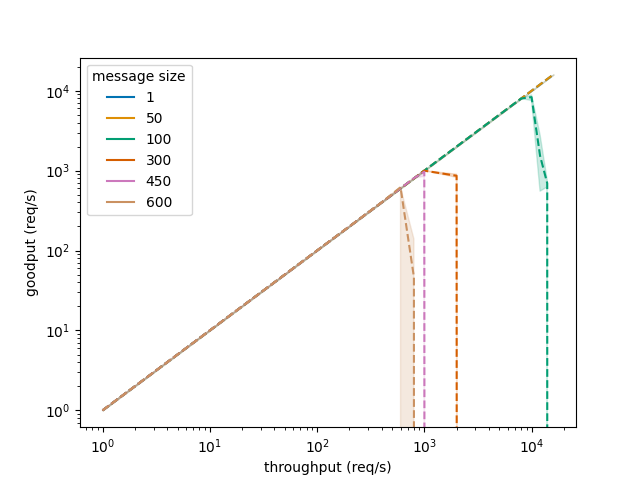
\includegraphics[scale=0.75]{dummy_test/throughputgoodput.png}
\caption{Benchmarking of Cap'n Proto server goodput for varying throughputs and message sizes.}
\end{figure}

\begin{figure}[h!]
\centering
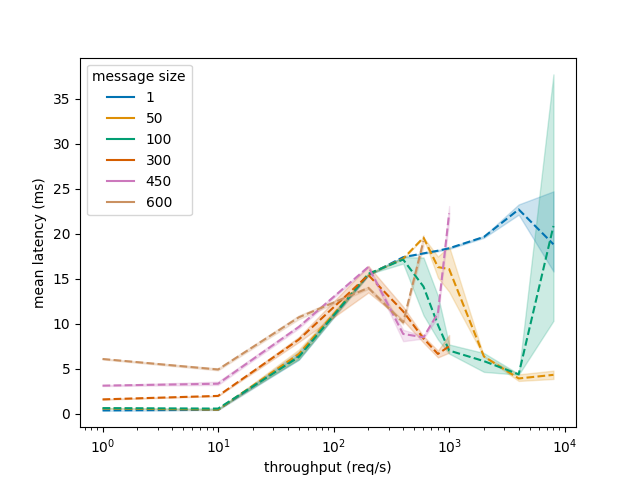
\includegraphics[scale=0.75]{dummy_test/throughputflatency.png}
\caption{Benchmarking of Cap'n Proto server latencies for varying throughputs and message sizes. Discarded result if goodput was not within 5\% of target throughput.}
\end{figure}

\begin{figure}[h!]
\centering
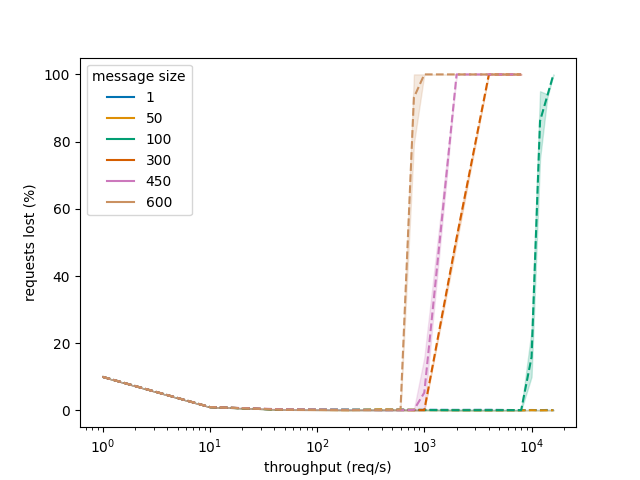
\includegraphics[scale=0.75]{dummy_test/throughputlost.png}
\caption{Benchmarking of Cap'n Proto server \% of failed requests for varying throughputs and message sizes, run for 10s}
\end{figure}

[describe the experiment methodology, present argument, then back up with evidence from figures]
We benchmarked the latency and goodput of sending messages in Cap'n Proto. We varied the size of messages sent in different tests to replicate the behaviour of the algorithm when sending `batches' of many commands, so a message size of 600 means that the message size is approximately that of a message containing 600 commands.

The figures demonstrate that the framework has a severe drop in performance when sending large messages. For a message size of 600 the goodput goes to zero as the throughput increases, meaning that no messages are being responded to.

[``Fundamentally, there are limitations in the RPC framework that give an upper bound on the performance we can hope to achieve, these limitations are evident in our benchmarking of the Cap'n Proto framework\dots'']

\subsection{Tezos Cryptography} \label{tezosbenchmark}
I profiled the important functions of the library with Jane Street's Core\_bench module [citation needed***]. Core\_bench is a micro-benchmarking library used to estimate the cost of operations in OCaml, it runs the operation many times and uses linear regression to try to reduce the effect of high variance between runs.

\begin{table}[!h]
	\centering
	\begin{tabular}{|l|r|}
	\hline
	Function                 & Time (µs) \\ \hline
	Sign                     & 427.87   \\
	Check                    & 1,171.77 \\
	Aggregate (4 sigs)       & 302.90   \\
	Aggregate check (4 sigs) & 1,179.25 \\
	Aggregate (8 sigs)       & 605.38   \\
	Aggregate check (8 sigs) & 1,180.61 \\ \hline
	\end{tabular}
	\caption{Benchmarking of key functions of the Tezos Cryptography library}
\end{table}
% ┌─────────────┬────────────┬─────────┬──────────┬──────────┬────────────┐
% │ Name        │   Time/Run │ mWd/Run │ mjWd/Run │ Prom/Run │ Percentage │
% ├─────────────┼────────────┼─────────┼──────────┼──────────┼────────────┤
% │ sign        │   427.87us │ 144.00w │          │          │     36.24  │
% │ check       │ 1_171.77us │  75.00w │          │          │     99.25  │
% │ agg_4       │   302.90us │ 484.00w │    0.15w │    0.15w │     25.66  │
% │ agg_check_4 │ 1_179.25us │  75.00w │          │          │     99.88  │
% │ agg_8       │   605.38us │ 944.00w │    0.35w │    0.35w │     51.28  │
% │ agg_check_8 │ 1_180.61us │  75.00w │          │          │    100.00  │
% └─────────────┴────────────┴─────────┴──────────┴──────────┴────────────┘

\section{HotStuff implementation benchmarks} \label{hotstuffbenchmarks}

\begin{figure}[h!]
\centering
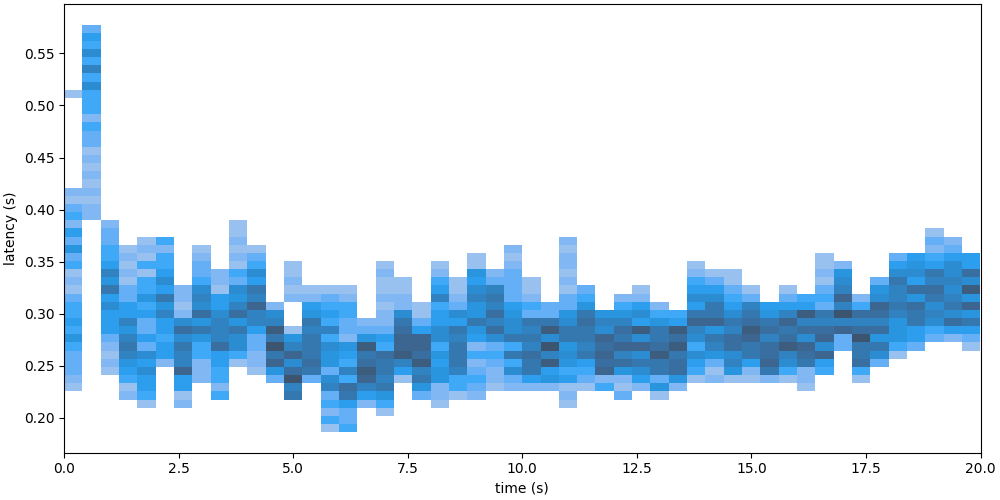
\includegraphics[scale=0.6]{heatmaps/batch_sizes_5_320_200_4_450_timelatencyheatmap.png}
\caption{Heatmap showing relatively stable latency throughout the course of the experiment. [add parameters!!]}
\label{stableheatmap}
\end{figure}

\begin{figure}[h!]
\centering
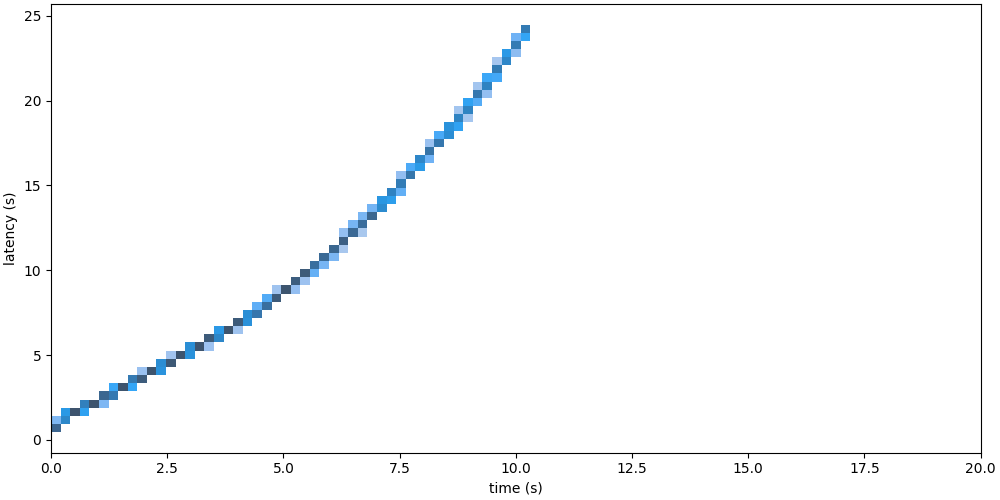
\includegraphics[scale=0.6]{heatmaps/batch_sizes_5_3_800_4_50_timelatencyheatmap.png}
\caption{Heatmap showing linear growth in latency as the experiment progresses. [add parameters]}
\label{linearheatmap}
\end{figure}

We now analyse the performance and behaviour of the system with different parameters, and under different conditions. We argue that the optimisations described in section \ref{performance} were effective in improving system performance, but there are fundamental limitations caused by the latency costs of Cap'n Proto serialisation (section \ref{capnpbenchmark}) and cryptography (section \ref{tezosbenchmark}).

In most cases, the system exhibits stable latency throughout an experiment while goodput is equal to throughput, meaning that the system is not overloaded (figure \ref{stableheatmap}). When the throughput exceeds the amount the system can keep up with, there is linear growth in latency as commands queue on the nodes (figure \ref{linearheatmap}). Since HotStuff is a partially synchronous protocol (section \ref{hotstufftheory}), an increase in latency means that view times increase, decreasing goodput. Once the system is overloaded, the goodput levels off at around its maximum value as throughput is increased.

In our comparison of batch sizes (section \ref{batchsizeseval}) there is evidence that the implementation of batching (section \ref{batching}) was effective, as the system is able to achieve much greater goodput with batch sizes greater than 1 (equivalent to no batching). This section also provides evidence that serialisation latency is a bottleneck, as view times begin to increase exponentially as batch sizes increase, due to messages being larger and taking longer to serialise.

Our study of node counts (section \ref{nodecountseval}) gives further evidence that message serialisation is a bottleneck; higher node counts mean more internal messages being sent, causing a decline in performance due to serialisation costs. This also supports the conclusion that cryptography is a bottleneck, as more nodes means more messages must be signed and aggregated.

In our ablation study (section \ref{ablation}) we compare the performance of the system with different optimisations enabled, demonstrating their effectiveness in increasing goodput, and lowering latency. We also demonstrate that cryptography is a bottleneck by demonstrating the superior performance of the system with cryptography disabled.

In our wide area network (WAN) simulation study (section \ref{minineteval}), we compare the performance of our system running locally, to a simulated mininet network (section \ref{testing}) with link latency similar to what one may observe in a wide area network. [we found...]

In our view-change study (section \ref{viewchange}) we demonstrate that the view-change protocol (section \ref{viewchange}) is effective in ensuring the system progresses once a node has died, albeit with a significant performance penalty.

\subsection{Batch sizes} \label{batchsizeseval}

\begin{figure}[h!]
\centering
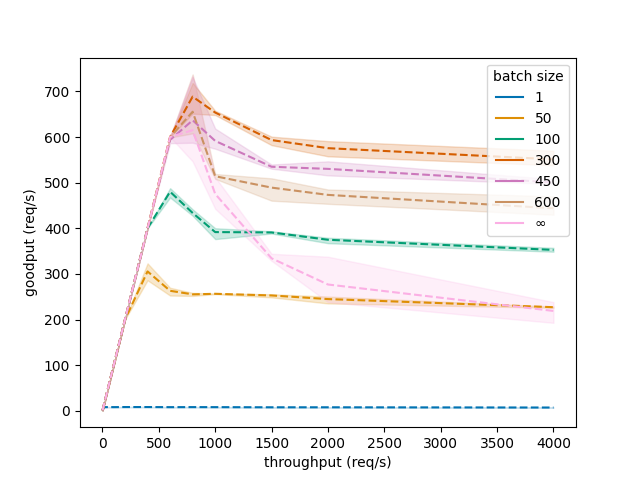
\includegraphics[scale=0.75]{batch_size_test/throughputgoodput.png}
\caption{Benchmarking of goodput for varying throughputs and batch sizes.}
\label{throughputgoodputbatch}
\end{figure}

\begin{figure}[h!]
\centering
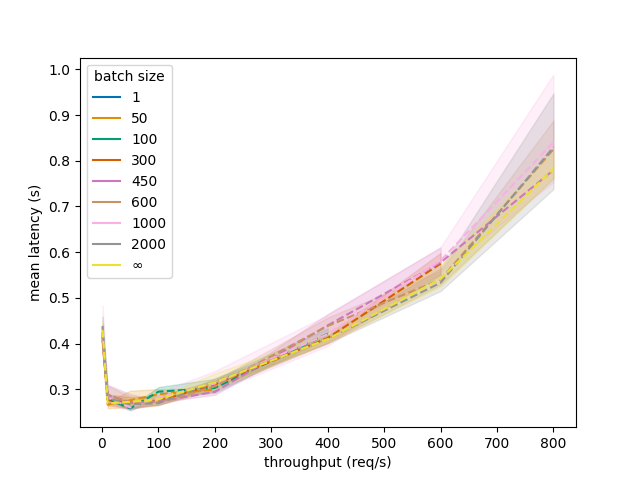
\includegraphics[scale=0.75]{batch_size_test/throughputflatency.png}
\caption{Benchmarking of mean latency while varying throughputs and batch sizes. Discarded result if goodput was not within 5\% of target throughput.}
\label{throughputlatencybatch}
\end{figure}

\begin{figure}[h!]
\centering
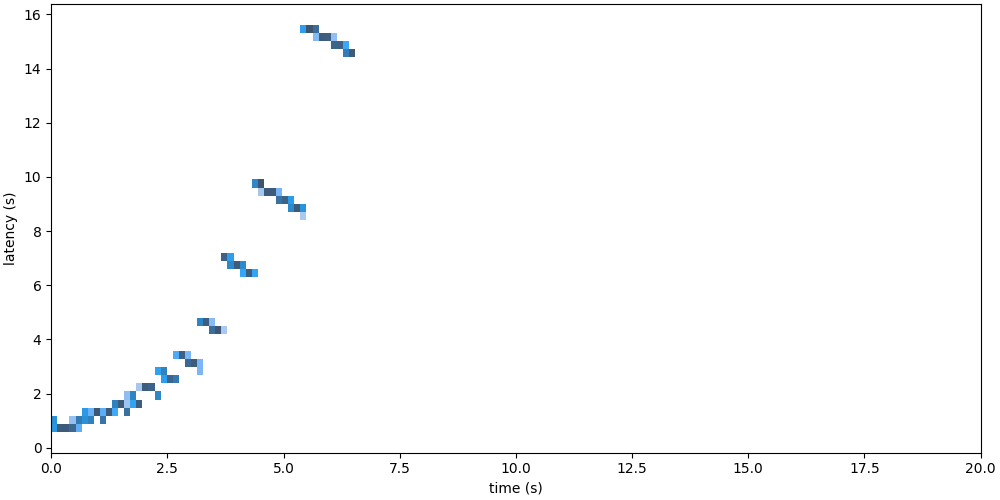
\includegraphics[scale=0.6]{heatmaps/batch_sizes_5_8_1800_4_99999999_timelatencyheatmap.png}
\caption{Heatmap showing exponential growth in latency as the experiment progresses. [add parameters]}
\label{expheatmap}
\end{figure}

This study compares the performance of the system for varying limits on batch sizes (section \ref{batchsizes}). All experiments were run on a network of 4 nodes.

At lower throughputs where the system is not overloaded, throughput grows linearly with goodput (figure \ref{throughputgoodputbatch}), as the system is able to respond to all incoming requests, with roughly constant latency throughout an experiment (figure \ref{stableheatmap}). During this period batches are not filled, so larger throughputs result in larger messages and a linear increase in latency due to increasing serialisation latency (figure \ref{throughputlatencybatch}). The system is able to reach a higher goodput before being overloaded if it has a larger batch size, as each view results in more commands being committed; this supports our conclusion that batching is an effective optimisation.

Once throughput is increased enough, batches begin to be filled up and the system is overloaded. This results in the goodput flattening out (figure \ref{throughputgoodputbatch}), as the system cannot handle the volume of requests; commands begin to queue on the nodes and latency increases linearly (figure \ref{linearheatmap}). For higher batch size limits (especially unlimited), goodput declines once the system is overloaded rather than flattening off. This is because the benefits of larger batches are offset by messages becoming larger, causing increased serialisation latency, which increase view times and lower goodput. For large batch sizes, view times increase exponentially, as shown by the growing vertical gaps between commands being committed in figure \ref{expheatmap}.

There is a clear trade-off between larger batch sizes that result in more commands being committed, and batches becoming too large and incurring exponential serialisation latency. The optimum for our system appears to be a batch size of around 600 commands, with a maximum goodput of around 900req/s. (figure \ref{throughputgoodputbatch}).

% There is a trade-off between having larger batches to process more commands, and messages becoming too large and increasing serialisation latency, which is apparent from figure \ref{throughputgoodputbatch}. With small batch sizes each view only commits a small number of commands, leading to low goodputs; an extreme example of this is a batch size of 1 (equivalent to no batching). As batch sizes increase the goodput reached also increases, with goodput peaking at around 700req/s with a batch size of 300 commands. At this point increasing batch size further causes goodput to decrease due to the increased latency of serialising large messages; each view takes longer so less nodes are committed per second (even though each node contains more commands). When the batch size is unlimited messages grow very large as throughput increases, and increased serialisation latency causes goodput to decline.

% Figure \ref{throughputlatencybatch} shows that latency scales linearly with throughput while the system is not overloaded, that is, when the goodput is within 5\% of the target throughput. This is because larger throughputs result in larger message sizes, and increased latency due to serialisation time. 

\subsection{Node counts} \label{nodecountseval}

\begin{figure}[h!]
\centering
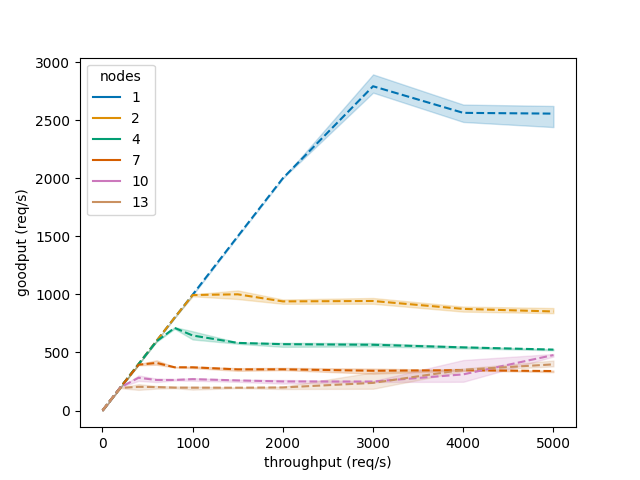
\includegraphics[scale=0.75]{node_count_test/throughputgoodput_nodes.png}
\caption{Benchmarking of goodput for varying throughputs and node counts.}
\label{throughputgoodputnodes}
\end{figure}

\begin{figure}[h!]
\centering
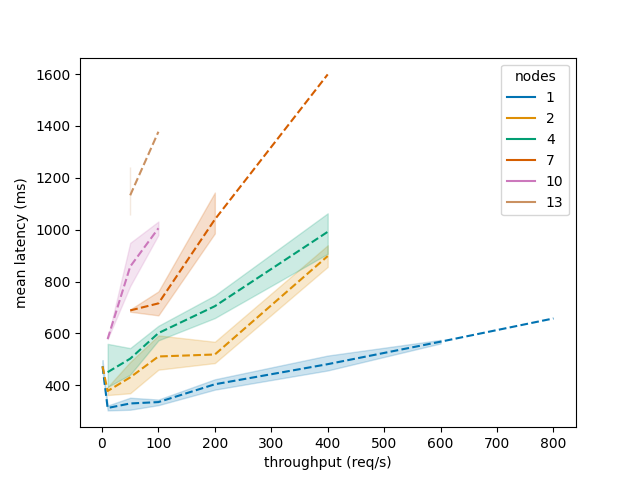
\includegraphics[scale=0.75]{node_count_test/throughputflatency_nodes.png}
\caption{Benchmarking of mean latency while varying throughputs and node counts. Discarded result if goodput was not within 5\% of target throughput.}
\label{throughputlatencynodes}
\end{figure}

This study compares the performance of the system for varying node counts. Node counts were chosen such that $n = 3f + 1$ for some $f$, as choosing another value would decrease performance without any benefit of increased fault-tolerance\footnote{A node count of 2 was also tested as it is the smallest node count where internal messages are exchanged.}. All experiments were run with a batch size of 300.

Figure \ref{throughputlatencynodes} shows that as node count increases, latency increases. This is because larger node counts mean that each view requires more internal messages to be sent to progress. Sending internal messages is expensive due to the latency of serialisation and cryptography, so this results in increased overall latency. Additionally, increasing the node count increases the number of messages that must be signed, and makes aggregating signatures slower (section \ref{tezosbenchmark}). As in our study of batch sizes (section \ref{batchsizeseval}), latency also increases linearly with throughput while the system is not overloaded. Notably the latency for a system of 1 node increases slowly, as there are no internal messages, just client requests and responses.

Figure \ref{throughputgoodputnodes} shows that the larger the node count, the lower the maximum goodput. This is again due to larger node counts resulting in more internal messages, causing more latency since this is a bottleneck. Increased latency causes each view to take longer, reducing the number of requests that can be responded to each second.

\subsection{Ablation study} \label{ablation}

\begin{table}[h]
\centering
\begin{tabular}{|c|c|c|c|c|}
\hline
Version & Chaining & Truncation & Filtering & Crypto \\ \hline
1 & \xmark & \xmark & \xmark & \cmark \\ \hline
2 & \cmark & \xmark & \xmark & \cmark \\ \hline
3 & \cmark & \xmark & \cmark & \cmark \\ \hline
4 & \cmark & \cmark & \xmark & \cmark \\ \hline
5 & \cmark & \cmark & \cmark & \cmark \\ \hline
6 & \cmark & \cmark & \cmark & \xmark \\ \hline
\end{tabular}
\caption{Features enabled in different versions.}
\label{versiontable}
\end{table}

\begin{figure}[h!]
\centering
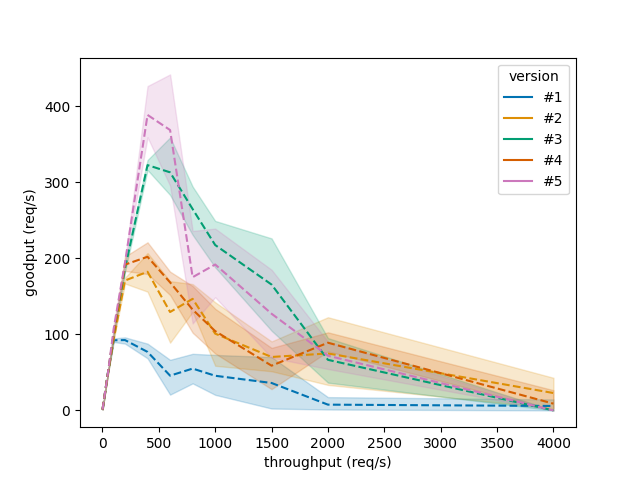
\includegraphics[scale=0.75]{ablation/throughputgoodput_ablation.png}
\caption{Benchmarking of goodput for varying throughputs and implementation versions, run for 10s with 4 nodes unlimited batch size.}
\label{throughputgoodputablation}
\end{figure}

\begin{figure}[h!]
\centering
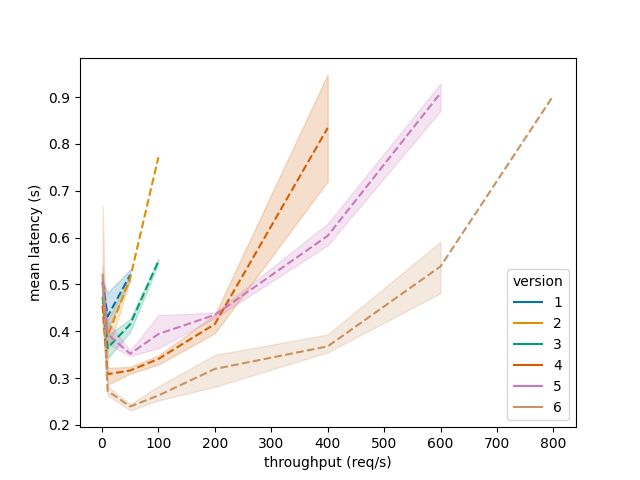
\includegraphics[scale=0.75]{ablation/throughputflatency_ablation.png}
\caption{Benchmarking of mean latency while varying throughputs and implementation versions, run for 10s with 4 nodes unlimited batch size. Discarded result if goodput was not within 5\% of target throughput.}
\label{throughputlatencyablation}
\end{figure}

This study compares the performance of different versions of the system with different optimisations enabled. The optimisations explored are chaining (section \ref{chaining}), node truncation (section \ref{truncation}), and command filtering (section \ref{filtering}). We also compare performance with, and without cryptography enabled. The mapping from version numbers to which features are enabled is given in table \ref{versiontable}. All experiments were run with a network of 4 nodes, and unlimited batch sizes.

\subsection{Wide area network simulation} \label{minineteval}

\begin{figure}[h!]
\centering
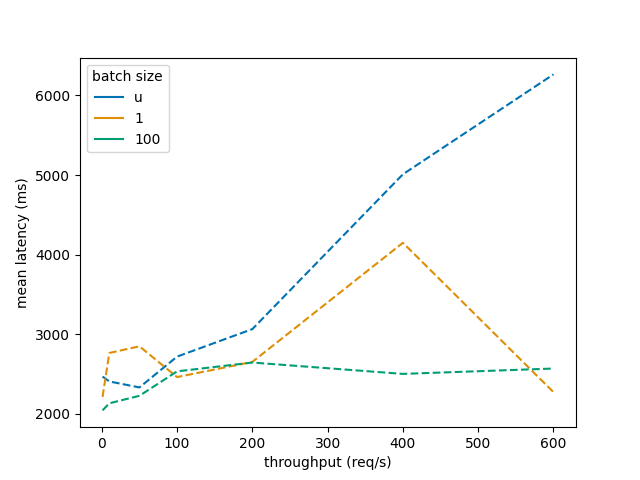
\includegraphics[scale=0.75]{mininet/throughputlatency.png}
\caption{Benchmarking of mean latency while varying throughputs and batch sizes, run for 10s with 100ms network delay.}
\end{figure}

\begin{figure}[h!]
\centering
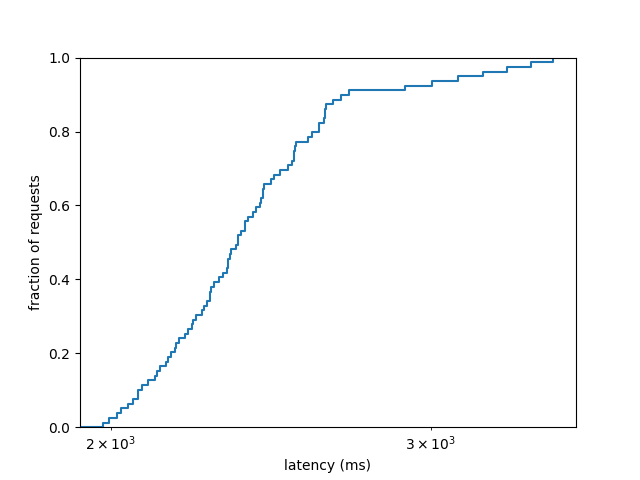
\includegraphics[scale=0.75]{mininet/10tpub_cumlatency.png}
\caption{Cumulative latency plot for experiment with a throughput of 10req/s and unlimited batch size, run for 10s with 100ms network delay.}
\end{figure}

[Give ablation graphs comparing the performance with 100ms delay, and without.]

\subsection{View-changes} \label{viewchangeeval}

\begin{figure}[h!]
\centering
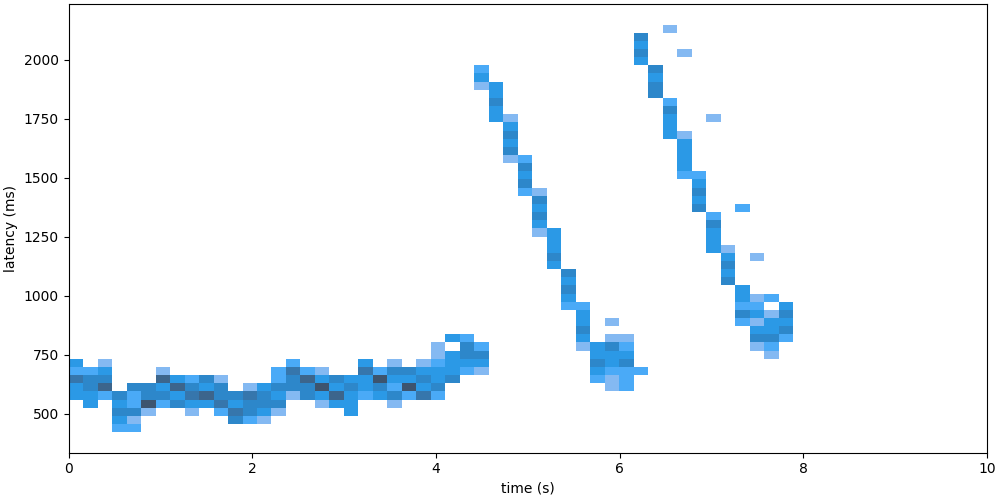
\includegraphics[scale=0.5]{viewchange/test7_100_7_100_timelatencyheatmap.png}
\caption{Heatmap showing distribution of latencies with a node being killed 5s in. Run for 10s with 7 nodes and a batch size of 100.}
\label{viewchangeheatmap}
\end{figure}

This study explores the behaviour of the system in the event of a node failing, where the view-change protocol (section \ref{viewchange}) is needed to skip the faulty leader's view and make progress.

Figure \ref{viewchangeheatmap} is a heatmap showing a node being killed 5s into an experiment. There is a clear jump in latency every time the killed node is the leader of the view, and the nodes must wait for the 0.5s timeout to elapse before the next view begins. The latency jump of around 1.25s is about what one would expect; 0.5s timeout and 0.75s of latency (the same as before the node was killed).

The view-change protocol is successful in allowing the system to make progress, albeit with a significant increase in latency. This is an inherent problem with the HotStuff protocol, although a failure-detector could help to minimise the number of views where the faulty node is leader.

% Clone github.com/cjen1/reckon

% ```
% # This is likely to take a while
% make reckon-mininet

% docker run -it --privileged -e DISPLAY --network host --name reckon-mininet cjen1/reckon:latest bash

% # Set up mininet net with a single switch and 3 nodes
% # drops you into a cli (you can also use python scripting)
% mn --topo single,3

% # observe no delay between nodes
% mininet> h1 ping h2
% mininet> <Ctrl-C>/<Ctrl-D> to exit

% # syntax is `mininet> <node> <command>`
% # I run screens on each node and then attach to those from outside mininet to run the tests in different terminal screens. (Tmux doesn't work correctly afaicr)

% mininet> h1 screen -dmS node_h1 bash

% #Then in another terminal session
% docker exec -it reckon-mininet bash
% screen -r node_h1
% <whatever commands you want to run on that emulated node>

% #Similarly for the other nodes
% ```

\stepcounter{chapter}
\chapter*{Conclusion}
\addcontentsline{toc}{chapter}{Conclusion}

% This chapter is likely to be very short and it may well refer back to the Introduction. It might offer a reflection on the lessons learned and explain how you would have planned the project if starting again with the benefit of hindsight.

% general-use framework ??
\section{Future Work}
Further work would port to using the async library which is known to have better performance. It was out of scope to rewrite in async or use it in the first place due to poor documentation (although now I could look at the type signatures and understand the documentation). Hopefully reimplementing would give better performance and avoid the bugs of capnrpc. I would carry out more extensive tests on the message sending capabilities before diving into implementation. I would be more aware beforehand of the whole algorithm (including the pacemaker code) and implement based on the new pseudocode we have presented and proven correct. This would allow for better structuring of the code.

% if i was to reimplement i would already have a solid grasp on the algorithm, language, and frameworks. i could focus more on the practicalities of bottlenecks, profiling, testing lwt & queueing, benchmarking, etc. from the outset

% to develop a real production ready system that has a reasonable level of performance would take an order of magnitude more time than this problem. one would have to carefully study byzantine threats and how one would counter availability attacks. In some cases optimisations may be antagonistic with security considerations (eg. TCP style truncation could be attacked). if the system was to be deployed in a real environment (eg. a cryptocurrency) security would be paramount, and it could take years of fixes and bug bounties to develop a robust system.

We have presented a potential path for implementing verifiable anonymous identities and reconfiguration using our permissioned blockchain, future work could consist of a practical implementation of this.

% \bibliographystyle{plain}
% \bibliography{references}
\bibliographystyle{acm}
\bibliography{ref}
% \printbibliography
\addcontentsline{toc}{chapter}{Bibliography}

\end{document}
